\chapter{Pomiarowa weryfikacja tezy}

Ostatni etap weryfikacji postawionej w pracy tezy stanowi analiza właściwości metrologicznych przykładowego toru pomiarowego, który stworzony został na potrzeby pracy. Analizowany tor pomiarowy przetwarza zmienny w czasie sygnał napięciowy $s(t)$ o chwilowej wartości napięcia z przedziału $<0;1>~\unit{V}$. W celu dopasowania poziomu sygnału napięcia wejściowego do zakresu napięcia wejściowego przetwornika analogowo-cyfrowego oraz zwiększenia impedancji wejściowej toru pomiarowego, sygnał $s(t)$ podawany jest na wejście wzmacniacza pomiarowego. Sygnał wyjściowy wzmacniacza $y(t)$ przetwarzany jest na postać cyfrową $c(i)$, a następnie po wykonaniu odtwarzania statycznego, podawany jest w postaci wielkości $x(i)$ na wejście jednostki \enquote{DSP}, która pobiera $N$ próbek tego sygnału i wyznacza na ich podstawie $M$ wartości wielkości wyjściowych toru pomiarowego, stosując w tym celu algorytm dyskretnej transformacji falkowej. Schemat blokowy omawianego toru pomiarowego przedstawiono na rysunku~\ref{fig:chain_real}.

\begin{figure}[htb!]
\begin{center}
\includegraphics{obrazki/schemat_real}
\makecaption{fig:chain_real}{Schemat blokowy stworzonego na potrzeby pracy toru pomiarowego będącego obiektem przeprowadzanego eksperymentu}
\end{center}
\end{figure}

Do realizacji układu wzmacniacza pomiarowego zastosowany został wzmacniacz operacyjny \enquote{MCP6002}~\cite{microchip_manual} w konfiguracji nieodwracającej, o docelowym wzmocnieniu wynoszącym~\qty{3.3}{V \per V}. Napięcie zasilania wzmacniacza wynosi~\qty{3.3}{V} i pochodzi ze stabilizatora \enquote{LD1117}~\cite{stm_manual} typu \enquote{LDO} (ang. \enquote{Low Dropout}). Zaproponowana konfiguracja, zgodnie z wcześniejszymi założeniami, zapewnia wysoką impedancję wejściową toru pomiarowego oraz bardzo niską impedancję wyjściową wzmacniacza. Parametry statyczne oraz dynamiczne analizowanego obiektu wymagają identyfikacji, ze względu na niedostateczne informacje zawarte w dokumentacji wykorzystanego układu oraz nieznajomości dokładnego modelu dla zastosowanej aplikacji. Należy zauważyć, że dokładna analiza zastosowanego układu byłaby skomplikowana i nie jest konieczna do oceny jego właściwości metrologicznych związanych z zastosowanie proponowanego w pracy modelu błędu.

Zastosowany przetwornik analogowo-cyfrowy stanowi $12$-bitowy przetwornik wagowy~\enquote{SAR} (ang. \enquote{Successive Approximation Register}), wbudowany w mikrokontroler \enquote{STM32F411}~\cite{stm_f411}. Źródło napięcia odniesienia stanowi w jego przypadku stabilizator \enquote{AP7343}~\cite{diodes_manual} typu \enquote{LDO}, o znamionowym napięciu wyjściowym równym~\qty{3.3}{V}, przyłączony z użyciem dodatkowego filtru LC. Przetwornik analogowo-cyfrowy taktowany jest wewnętrznym sygnałem zegarowym o częstotliwości~\qty{24}{MHz}, przy czym próbkowanie wyzwalane jest sygnałem z licznika, którego częstotliwość wyzwalania wynosi~\qty{48}{kHz}. Częstotliwość próbkowania analizowanego toru pomiarowego wynosi zatem $f_{s} = \qty{48}{kHz}$. Na proces konwersji analogowo-cyfrowej przypada proces kluczowania napięcia wejściowego trwający $15$ taktów zegara, po którym następuje konwersja trwająca $15$ taktów zegara, co w analizowanym przypadku stanowi czas~\qty{625}{ns} dla każdej z operacji. Łączny czas konwersji analogowo-cyfrowej pojedynczej próbki sygnału wejściowego $y(t)$ na jego dyskretną reprezentację $c(i)$ wynosi zatem~\qty{1250}{ns}. Ze względu na typową aplikacje omawianego przetwornika, jego parametry metrologiczne mogą zostać pozyskane z dokumentacji producenta układu~\cite{stm_f411}.

Pozyskane próbki napięcia $x(i)$, stanowiące dyskretną reprezentację sygnału wejściowego $s(t)$, zapisywane są w wektorze $\mathbf{x}$ o długości $N = 128$. Wektor wielkości wejściowych $\mathbf{x}$ podawany jest na wejście algorytmu dyskretnej transformacji falkowej, którego implementacja zrealizowana została z wykorzystaniem instrukcji \enquote{DSP} dostępnych dla zastosowanego mikrokontrolera~\cite{reay_dsp}. Analizowany algorytm wykorzystuje falkę \enquote{spline4:4}~\cite{wang_splinebasics} dla pięciu iteracji procesu dekompozycji sygnału. Zgodnie z równaniem~\eqref{eq:alg_out_mat} wyznaczanych jest $M = 128$ próbek wektora wielkości wyjściowych $\mathbf{X}$, które stanowią wyjście dla pojedynczej serii pomiarowej analizowanego toru pomiarowego. Wartości elementów macierzy transformacji $\mathbf{A}$ zidentyfikowano zgodnie z metodoą przedstawioną w równaniu~\eqref{eq:wt_ident}, wykorzystując w tym celu implementacje algorytmu transformacji falkowej dostępną w programie \enquote{GNU Octave}~\cite{pruuvsa_dwt}. Czas obliczeń wynosi w analizowanym przypadku~\qty{1508}{\micro s}, przy czym łączny czas akwizycji pojedynczego wektora próbek wielkości wejściowych wynosi~\qty{2666.6(6)}{\micro s}. Podczas obliczeń stosowane są liczby zmiennoprzecinkowe o długości słowa $32$-bitów.

Przedstawiony tor pomiarowy pracuje w trybie ciągłym, tj. w pojedynczym oknie pomiarowym, podczas pobierania próbek wielkości wejściowych wektora $\mathbf{x}$, wyznaczana jest realizacja wektora wielkości wyjściowych $\mathbf{X}$ dla poprzedniej realizacji wektora wielkości wejściowych. Wykorzystywany jest w tym celu kontroler \enquote{DMA} (ang. \enquote{Direct Memory Access}), nadzorujący proces buforowania kolejnych realizacji sygnału $x(i)$, w czasie gdy program główny wykonuje obliczenia dane równaniem~\eqref{eq:alg_out_mat}. Analiza wartości wielkości wyjściowych omawianego toru pomiarowego jest możliwa między innymi po podłączeniu go do komputera klasy \enquote{PC} za pośrednictwem portu \enquote{USB}, przy czym wykorzystywany jest w tym celu układ peryferyjny \enquote{USB OTG Full-Speed}, zintegrowany w zastosowanym mikrokontrolerze.

W dalszej części rozdziału opisano najważniejsze źródła błędów analizowanego toru pomiarowego, a następnie wykorzystano zaproponowany w pracy model błędu do opisu właściwości wykazanych sygnałów błędów. Ze względu na fakt, że nie jest znany dokładny model analizowanego toru pomiarowego, przeprowadzono identyfikację jego właściwości, istotnych ze względu na zaproponowany model błędu. W ostatniej części rozdziału opisano przeprowadzony eksperyment pomiarowy, wykorzystujący metodę Monte-Carlo, mający na celu ocenę poprawności przedstawionych rozważań i weryfikacje możliwości praktycznej aplikacji zawartych w pracy propozycji. Temperatura otoczenia podczas przeprowadzania eksperymentów była stała i wynosiła~\qty{21}{\degreeCelsius}.

\section{Identyfikacja właściwości toru pomiarowego}

Pierwszą grupą identyfikowanych właściwości analizowanego toru pomiarowego będą jego właściwości statyczne. Właściwości te nie zależą od częstotliwości przetwarzanego sygnału i wynikać będą z charakterystyk przetwarzania statycznego kolejnych fragmentów tego toru. Jako, że z punktu widzenia przeprowadzanej analizy właściwości metrologicznych oraz właściwości zaproponowanej w pracy metody analizy, najistotniejsze informacje stanowić będą dane dotyczące parametrów sygnałów błędów na wejściu algorytmu dyskretnej transformacji falkowej, najbardziej przystępne z punktu widzenia projektanta toru pomiarowego będzie wyznaczenie tych parametrów traktując całość toru pomiarowego znajdującego się przed tym algorytmem, jak jeden obiekt.

Wobec powyższych, proponuje się wyznaczenie charakterystyki statycznej $f_{c}(x)$ dla wielkości wyjściowej $c(i)$ przetwornika analogowo-cyfrowego, a następnie na jej podstawie określenie funkcji odtwarzania $f_{x}(x)$. Należy w tym celu na wejście toru pomiarowego podawać, z wzorcowego źródła napięcia, napięcie stałe o zadanej wartości, a następnie pobierać wielokrotnie wartość realizacji wielkości wyjściowej $\hat{c}(i)$ przetwornika analogowo-cyfrowego, którą następnie należy uśrednić dla przeprowadzonej serii pomiarów. Podczas eksperymentu na wejście toru pomiarowego podawano napięcie stałe z zakresu $<0;1>~\unit{V}$ z krokiem wynoszącym~\qty{12.5}{mV}, a na pojedynczą serię pomiarową składało się trzydzieści tysięcy próbek wielkości wyjściowej przetwornika analogowo-cyfrowego. Źródło napięcia wejściowego stanowił w przeprowadzonym eksperymencie kalibrator FLUKE 5700A~\cite{fluke_manual}, stąd założyć można, że przetwarzany sygnał $s(t)$ nie zawierał żadnych sygnałów błędów, a zatem wszystkie sygnały błędów obecne w torze pomiarowym stanowiły błędy własne tego toru.

Na podstawie przeprowadzonych pomiarów, po wykonaniu aproksymacji liniowej stosując metodę najmniejszych kwadratów, funkcję przetwarzania analizowanego obiektu opisać można równaniem:
\begin{equation}
c \emb{i} = f_{c} \emb{f_{y} \emb{s \emb{iT_{p}}}} = 4.0956 \cdot s \emb{iT_{p}} + 4.1764 \label{eq:pom_func_static}.
\end{equation}
Zakładając, że czułość wielkości $x(i)$ w stosunku do wielkości $s(t)$ wynosi~\qty{1}{V \per V}, funkcję odtwarzania statycznego wielkości $x(i)$ na podstawie wielkości $c(i)$ można opisać jako:
\begin{equation}
x \emb{i} = f_{x} \emb{f_{c} \emb{f_{y} \emb{s \emb{iT_{p}}}}} = \frac{c \emb{i} - 4.1764}{4.0956} = s \emb{iT_{p}} \label{eq:pom_funx_static}.
\end{equation}
Odchylenie standardowe średnich wartości $\overline{c}(i)$ uzyskanych dla kolejnych serii pomiarowych od charakterystyki danej równaniem~\eqref{eq:pom_func_static} wyniosło $\sigma_{c,l} = \qty{0.56}{kwantu}$, co interpretować można jako niepewność standardową nieliniowości charakterystyki statycznej przetwarzania wielkości $c(i)$. Po wykonaniu odtwarzania statycznego, zgodnie z równaniem~\eqref{eq:pom_funx_static}, niepewność standardowa związana z nieliniowością charakterystyki odtwarzania wielkości $x(i)$ wynosi odpowiednio $\sigma_{x,l} = \qty{0.14}{mV}$.

Poza nieliniowością charakterystyki odtwarzania sygnału $x(i)$ w budżecie niepewności uwzględnić należy występowanie pozostałych czynników zakłócających proces pomiaru. Czynniki te stanowią między innymi zakłócenia wynikające z fluktuacji napięcia zasilania wzmacniacza pomiarowego oraz napięcia odniesienia przetwornika analogowo-cyfrowego, błędy kwantowania, niejednorodność wzorców struktury wewnętrznej przetwornika analogowo-cyfrowego, czy szumy występujące w części analogowej toru pomiarowego. Jako, że z punktu widzenia proponowanego w pracy modelu błędu, istotne są jedynie parametry wypadkowego sygnału błędu $e_{x}(i)$ opisanego równaniem:
\begin{equation}
e_{x} \emb{i} = \tilde{x} \emb{i} - \dot{s} \emb{iT_{p}} \label{eq:pom_funx_error},
\end{equation}
parametry te można zidentyfikować na podstawie przeprowadzonego eksperymentu. Definiując sygnał błędu $e_{c}(i)$ w postaci:
\begin{equation}
e_{c} \emb{i} = \tilde{c} \emb{i} - f_{c} \emb{f_{y} \emb{\dot{s} \emb{iT_{p}}}} \label{eq:pom_func_error},
\end{equation}
istnieje możliwość sporządzenia na podstawie wykonanych pomiarów histogramu, a następnie zgodnie z równaniem~\eqref{eq:unc_summation} wyznaczenia niepewności rozszerzonej związanej z sygnałem błędu $e_{c}(i)$. Oszacowana wartość niepewności $U_{c,s}$ związana z właściwościami statycznymi analizowanego fragmentu toru pomiarowego wyniosła $U_{c,s} = \qty{2.54}{kwantu}$. Biorąc pod uwagę zależność daną równaniem~\eqref{eq:pom_funx_static} niepewność związana z sygnałem błędu $e_{x}(i)$ w analizowanym przypadku właściwości statycznych wynosi odpowiednio $U_{x,s} = \qty{0.62}{mV}$. Wyniki pomiarów wielkości $\overline{c}(i)$ w funkcji napięcia wejściowego dla przeprowadzonych serii pomiarowych oraz histogram uzyskanych realizacji sygnału błędu $e_{c}(i)$ przedstawiono na rysunku~\ref{fig:pom_static_fun}.

\begin{figure}[htb!]
\begin{center}
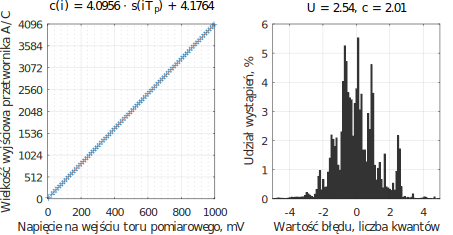
\includegraphics{obrazki/static_adcout}
\makecaption{fig:pom_static_fun}{Zależność wartości wielkości wyjściowej przetwornika analogowo-cyfrowego w funkcji wartości napięcia wejściowego analizowanego toru pomiarowego oraz histogram uzyskanych realizacji błędu statycznego wielkości wyjściowej przetwornika analogowo-cyfrowego}
\end{center}
\end{figure}

Należy zaznaczyć, że z punktu widzenia proponowanego modelu błędu dokładna znajomość postaci funkcji przetwarzania statycznego każdego elementu toru pomiarowego nie jest znana. Przykładowo, pomimo udziału funkcji przetwarzania $f_{y}(x)$ wzmacniacza pomiarowego w równaniach~\eqref{eq:pom_func_static} oraz~\eqref{eq:pom_funx_static}, znajomość tej funkcji nie jest konieczna podczas omawianej analizy. Dodatkowo, na podstawie treści przedstawionych równań zauważyć można, że na etapie przetwarzania wielkości $c(i)$ wprowadzane jest przesunięcie charakterystyki statycznej, które najprawdopodobniej spowodowane jest błędem zera wzmacniacza pomiarowego. Opisywana sytuacja powoduje, że funkcja przetwarzania nie spełnia właściwości addytywności, przez co nie jest możliwa analiza każdego sygnału błędu z osobna, jak proponowano w opisanym w pracy modelu błędu. Przeprowadzenie analizy z punktu widzenia wielkości wejściowej algorytmu dyskretnej transformacji falkowej umożliwia eliminację opisywanych niedogodności i wykorzystanie równań od~\eqref{eq:out_disc_err_stat_self} do~\eqref{eq:out_disc_err_rand_prop}, umożliwiających analizę z zastosowaniem metody superpozycji dla obecnych w torze pomiarowym sygnałów błędów.

Analizując dokumentacje~\cite{microchip_manual, stm_manual, diodes_manual, stm_f411} kolejnych komponentów toru pomiarowego zauważyć można, że najistotniejsze źródło błędów związanych z właściwościami statycznymi stanowi w analizowanym przypadku przetwornik analogowo-cyfrowy. Zgodnie z dokumentacją~\cite{stm_f411}, typowa wartość błędu granicznego wielkości wyjściowej $c(i)$ dla zbliżonych do stosowanych w sporządzonej aplikacji parametrów pracy przetwornika analogowo-cyfrowego powinna mieścić się w przedziale $\pm<2; 3>~\unit{LSB}$, co pokrywa się z wartością uzyskaną na podstawie histogramu przedstawionego na rysunku~\ref{fig:pom_static_fun}. Najważniejsze źródła błędu, które zdefiniowane są przez producenta zastosowanego przetwornika analogowo-cyfrowego obejmują: błąd przesunięcia charakterystyki względem zera, błąd wzmocnienia, całkowy błąd nieliniowości i różnicowy błąd nieliniowości~\cite{stm_adc}. Przeprowadzony eksperyment pozwolił zidentyfikować wypadkowe parametry sumy opisanych sygnałów błędów, przy czym należy zauważyć, że ze względu niewielką w stosunku do rozdzielczości przetwornika liczbę serii pomiarowych, nie udało się uzyskać większości realizacji różnicowego błędu nieliniowości. Na podstawie wyników eksperymentu oraz informacji zawartych w dokumentach~\cite{stm_f411, stm_adc} można jednak przyjąć, że niepewność $U_{c}$ została oszacowana prawidłowo, przy czym ze względu na niewielką liczbę realizacji różnicowego błędu nieliniowości można zakładać, że rzeczywisty rozkład błędu $e_{c}(i)$ będzie rozkładem normalnym.

Drugą grupą koniecznych do identyfikacji właściwości są właściwości dynamiczne. Podobnie, jak w przypadku właściwości statycznych, istnieje możliwość ich identyfikacji pomiarowej uzyskując kolejne realizacje wielkości wyjściowej $c(i)$. Przypadek właściwości dynamicznych jest jednak złożony i wymaga stosowania bardziej skomplikowanej procedury pomiarów -- konieczna bowiem jest odpowiednia synchronizacja przebiegu napięcia wejściowego toru pomiarowego z przebiegiem sygnału wyjściowego przetwornika analogowo-cyfrowego, w celu oszacowania różnicy pomiędzy fazami analizowanych sygnałów. Opisywana procedura byłaby zatem kłopotliwa, a dodatkowo podczas jej realizacji wprowadzany byłby kolejny błąd, związany z opisywaną synchronizacją. Wobec powyższych okoliczności proponuje się w pierwszej kolejności identyfikację właściwości dynamicznych zastosowanego wzmacniacza pomiarowego, a następnie ustalenie właściwości dynamicznych przetwornika analogowo-cyfrowego na podstawie jego dokumentacji~\cite{stm_f411}, która szczegółowo opisuje model tego przetwornika.

W przypadku wzmacniacza pomiarowego procedura identyfikacji polega na podawaniu na jego wejście napięcia sinusoidalnie zmiennego, o zadanej częstotliwości i stałej amplitudzie. Dla zadanych parametrów sygnału zmierzyć należy amplitudę sygnału wyjściowego wzmacniacza, potrzebną do wyznaczenia jego wzmocnienia $K_{y}(f)$, oraz przesunięcie fazowe $\varphi_{y}(t)$ pomiędzy sygnałem wejściowym $s(t)$ i wyjściowym $y(t)$, przy czym pomiędzy omawianymi wielkościami zachodzą następujące relacje:
\begin{gather}
K_{y} \emb{f} = 20 \log \left( \frac{A_{wy} \emb{f}}{A_{we} \emb{f}} \right) \label{eq:pom_dyn_amp}, \\
\varphi_{y} \emb{f} = \varphi_{wy} \emb{f} - \varphi_{we} \emb{f} \label{eq:pom_dyn_phi},
\end{gather}
gdzie $A_{wy}(f)$ jest amplitudą sygnału wyjściowego, $A_{we}(f)$ amplitudą sygnału wejściowego, $\varphi_{wy}(f)$ przesunięciem fazowym sygnału wyjściowego, natomiast $\varphi_{we}(f)$ przesunięciem fazowym sygnału wejściowego wzmacniacza w funkcji częstotliwości.

Na podstawie pozyskanych danych oszacować można pasmo przenoszenia analizowanego wzmacniacza, które w tym przypadku wyniosło $f_{y,g} = \qty{123}{kHz}$. Dla przedstawionych charakterystyk sporządzono dwa modele aproksymacji. W modelu pierwszym wykorzystano funkcję opisującą transmitancję wzmacniacza w postaci:
\begin{gather}
\tilde{G}_{y} \emb{j\omega} = \frac{1}{1 + j \frac{\omega}{2 \pi f_{y,g}}} = \frac{1}{\frac{\omega^{2}}{4 \pi^{2} f_{y,g}^{2}} + 1} - j \frac{\omega}{2 \pi f_{y,g} \left( \frac{\omega^{2}}{4 \pi^{2} f_{y,g}^{2}} + 1 \right) } \label{eq:pom_dyn_trans},
\end{gather}
natomiast dla modelu drugiego wykonano metodą najmniejszych kwadratów aproksymacje wielkości danych równaniami~\eqref{eq:pom_dyn_amp} oraz~\eqref{eq:pom_dyn_phi} przy użyciu wielomianów:
\begin{gather}
K_{y} \emb{f} = 123 \cdot f^{2} - 321 \cdot f \label{eq:pom_aprox_amp}, \\
\varphi_{y} \emb{f} = 123 \cdot f^{2} - 321 \cdot f \label{eq:pom_aprox_phi}.
\end{gather}
Uzyskane dla zakresu częstotliwości $<0.1;300>~\unit{kHz}$ wartości wzmocnienia i przesunięcia fazowego oraz odpowiadające im wartości dla zaproponowanych w równaniach od~\eqref{eq:pom_dyn_trans} do~\eqref{eq:pom_aprox_phi} przedstawiono na rysunkach~\ref{fig:pom_dynamic_amp} oraz~\ref{fig:pom_dynamic_phi}.

Analizując przedstawione wykresy zauważyć można, że model zaproponowany w równaniach~\eqref{eq:pom_aprox_amp} oraz~\eqref{eq:pom_aprox_phi} stanowi bardzo dobre przybliżenie charakterystyki analizowanego wzmacniacza pomiarowego, natomiast model dany równaniem~\eqref{eq:pom_dyn_trans} odbiega od niej znacząco. Stąd przyjmuje się, że omawiane równania~\eqref{eq:pom_aprox_amp} oraz~\eqref{eq:pom_aprox_phi} opisywać będą właściwości dynamiczne zastosowanego wzmacniacza, odpowiadające zależnościom~\eqref{eq:mid_cont_amp} oraz~\eqref{eq:mid_cont_phi}. Należy zauważyć, że na potrzeby zaproponowanego w pracy modelu błędu informacje te będą wystarczające i nie jest konieczna znajomość dokładnej postaci funkcji opisującej transmitancję analizowanego obiektu.

Stosowanym podczas eksperymentu źródłem napięcia wielkości wejściowej $s(t)$ był generator przebiegów arbitralnych RIGOL~DG1011~\cite{rigol_manual}.

\begin{figure}[htb!]
\begin{center}
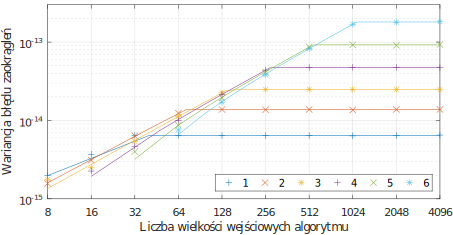
\includegraphics{obrazki/dwt_rerror_coif5}
\makecaption{fig:pom_dynamic_amp}{Zależność wartości wzmocnienia w funkcji częstotliwości dla zastosowanego w torze pomiarowym wzmacniacza}
\end{center}
\end{figure}

\begin{figure}[htb!]
\begin{center}
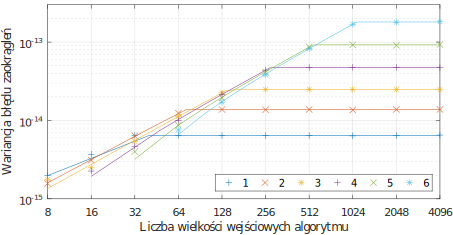
\includegraphics{obrazki/dwt_rerror_coif5}
\makecaption{fig:pom_dynamic_phi}{Zależność wartości przesunięcia fazowego w funkcji częstotliwości dla zastosowanego w torze pomiarowym wzmacniacza}
\end{center}
\end{figure}

Zgodnie z dokumentacją~\cite{stm_f411} obwód zastępczy części analogowej przetwornika analogowo-cyfrowego przedstawić można w postaci modelu filtra dolno-przepustowego typu \enquote{RC}, przy czym stanowić on będzie kaskadowe połączenie dwóch takich filtrów, co przedstawiono na rysunku~\ref{fig:schemat_adc}. Wypadkowa pojemność $C_{we}$ wynika w analizowanym przypadku z pojemności w obrębie wyprowadzenia mikrokontrolera, natomiast pojemność $C_{adc}$ wynika pojemności wewnętrznej układu próbkująco-pamiętającego. Zgodnie z dokumentacją wewnętrzna pojemność przetwornika wynosi typowo około~\qty{4}{pF}, natomiast pojemność zastępcza $C_{we}$ obwodu wejściowego przetwornika wynosi zwykle około~\qty{5}{pF}. Rezystancję $R_{we}$ w zaproponowanym modelu stanowi szeregowe połączenie rezystancji doprowadzeń pomiędzy wzmacniaczem pomiarowym i mikrokontrolerem oraz rezystancja samego wzmacniacza, przy czym w omawianym przypadku jest to wartość rzędu pojedynczych Ohmów. Rezystancja $R_{adc}$ jest rezystancją klucza układu próbkująco-pamiętającego i, zgodnie z dokumentacją, jej wartość nie przekracza~\qty{6}{k\ohm}. Dodatkowe elementy, które można zauważyć na omawianym schemacie, to diody zabezpieczające wejście mikrokontrolera przed zbyt wysokim lub niskim napięciem wejściowym oraz źródło $I_{adc}$, które zastępuje upływność układu nieprzekraczającą~\qty{\pm 1}{\micro A}. Elementy te mogą być zatem pominięte w omawianej analizie, ze względu na ich znikome znaczenie w budżecie błędów analizowanego toru pomiarowego.

\begin{figure}[htb!]
\begin{center}
\includegraphics{obrazki/schemat_adc}
\makecaption{fig:schemat_adc}{Schemat zastępczy modelu przetwornika analogowo-cyfrowego zastosowanego w analizowanym torze pomiarowym zgodny z dokumentacją producenta układu~\cite{stm_f411}}
\end{center}
\end{figure}

Pierwszy filtr, który przedstawiono na rysunku~\ref{fig:schemat_adc}, składa się z rezystancji rzędu pojedynczych Ohmów oraz pojemności rzędu mikro Faradów. Pozwala to oszacować częstotliwość graniczną tego filtru na poziomie kilkuset giga Herców. Filtr drugi stanowi połączenie rezystancji rzędu kilo Ohmów z pojemnością rzędu piko Faradów, a zatem rząd wielkości częstotliwości granicznej takiego filtru oszacować można na poziomie kilkuset mega Herców. Na podstawie przedstawionych parametrów modelu analizowanego przetwornika analogowo-cyfrowego, przyjąć można pomijalnie mały udział jego właściwości dynamicznych w puli właściwości dynamicznych całego toru pomiarowego. Ostateczna analiza właściwości dynamicznych całości toru pomiarowego uwzględniać będzie zatem tylko właściwości zastosowanego wzmacniacza pomiarowego, którego pasmo przenoszenia cechowało się wartością rzędu kilkuset kilo Herców.

Ostatnim fragmentem toru pomiarowego, który wprowadzać może do sygnału wyjściowego dodatkowe błędy, jest algorytm dyskretnej transformacji falkowej. Jako, że zastosowany mikrokontroler posiada jednostkę \enquote{FPU} (ang. \enquote{Floating Point Unit}) oraz zestaw instrukcji \enquote{DSP} umożliwiające optymalne wykonywanie operacji na liczbach zmiennoprzecinkowych pojedynczej precyzji, wykorzystane zostaną liczby o długości słowa $32$-bitów. Przeprowadzone wcześniej badania, których wyniki przedstawiono w tabeli~\ref{tab:varnum_spline4_4_5_f32}, pozwalają przypuszczać, że wariancja błędu związanego z zaokrągleniami nie przekroczy w bieżącym przypadku rzędu piko Voltów, a zatem niepewność rozszerzona z nią związana nie powinna przekroczyć rzędu mikro Voltów.

Dotychczasowe rozważania zakładały, że podawany na wejście toru pomiarowego z zastosowanego generatora sygnał cechował się idealną wartością napięcia. W rzeczywistości sygnał ten również obarczony był pewnym błędem, który zostanie uwzględniony i opisany w kolejnym podrozdziale. Przedstawione dotychczas zabiegi umożliwią sporządzenie modelu błędu analizowanego toru pomiarowego w oparciu o model błędu przedstawiony w niniejszej pracy.

\section{Model błędu toru pomiarowego}

Zakładając dla wielkości wejściowej $x(i)$ algorytmu dyskretnej transformacji falkowej czułość równą~\qty{1}{V \per V} w stosunku do przetwarzanego sygnału $s(t)$, idealny przebieg wielkości $x(i)$ opisać można w postaci:
\begin{equation}
\dot{x} \emb{i} = \dot{f}_{x} \left( \dot{f}_{c} \left( \dot{f}_{y} \left( s \emb{kT_{p}} \right) \right) \right) = \dot{s} \emb{kT_{p}} \label{eq:pom_dwtina_ideal},
\end{equation}
wobec czego, przy założeniu czułości wzmacniacza równej~\qty{3.3}{V \per V} oraz idealnej charakterystyki przetwarzania przetwornika analogowo-cyfrowego, idealne funkcje przetwarzania kolejnych fragmentów toru pomiarowego opisują równania:
\begin{gather}
\dot{f}_{y} \emb{x} = 3.3 \cdot x \label{eq:pom_ampfun_ideal}, \\
\dot{f}_{c} \emb{x} = 4096 \cdot \frac{x}{3.3} \label{eq:pom_adcfun_ideal}, \\
\dot{f}_{x} \emb{x} = \frac{x}{4096} \label{eq:pom_confun_ideal}.
\end{gather}

Przeprowadzone wcześniej pomiary, których wynik przedstawiono na rysunku~\ref{fig:pom_static_fun}, wykazują jednak pewne rozbieżności pomiędzy założeniami danymi w równaniach~\eqref{eq:pom_ampfun_ideal} oraz~\eqref{eq:pom_adcfun_ideal}. Omawiane różnice wynikają z innych niż zakładano parametrów czułości wzmacniacza pomiarowego, wartości napięcia referencyjnego lub wartości napięcia zasilania wzmacniacza. Ze względu na fakt, że przedstawiony tor pomiarowy występuje w formie prototypu, który nie będzie produkowany seryjnie, przyjmuje się że pomiar zakłócany jest błędami systematycznymi, niezmiennymi w czasie, które należy skorygować. Proponuje się zatem na podstawie pozyskanych wcześniej wyników pomiarów opisać ogólną funkcję przetwarzania wielkości $s(t)$ na wielkość $c(i)$, na podstawie której opisana zostanie odwrotna do niej funkcja odtwarzania wielkości $x(i)$ uwzględniająca wprowadzone korekty. Wobec powyższych zapisać można równania:
\begin{gather}
\dot{f}_{sc} \emb{x} = 4096 \cdot \frac{x}{1234} \label{eq:pom_scfun_ideal}, \\
\dot{f}_{cx} \emb{x} = \frac{x}{4096} \label{eq:pom_cxfun_ideal}, \\
\dot{f}_{sx} \emb{x} = \dot{f}_{cx} \left( \dot{f}_{sc} \emb{x} \right) \label{eq:pom_sxfun_ideal}, \\
\dot{x} \emb{i} = \dot{f}_{sx} \left( s \emb{kT_{p}} \right) \label{eq:pom_dwtinb_ideal},
\end{gather}
przy czym należy zauważyć, że sens równania~\eqref{eq:pom_dwtina_ideal} zostaje zachowany. W przypadku, gdyby analizowany tor pomiarowy miał być produkowany seryjnie, należałoby wskazać niepewność standardową dla wartości napięcia referencyjnego oraz czułości statycznej zastosowanego wzmacniacza, a następnie korzystając z prawa propagacji niepewności opisanego w~\cite{jcgm_guide} wyznaczyć niepewność związaną z rozrzutem tych parametrów.



\section{Weryfikacja przedstawionych zależności}

TODO

\section{Podsumowanie przeprowadzonego eksperymentu}

TODO

